\subsection{Experiments} 

The in-depth code implementation of the experiment run in this section can be found in the \textit{ReClassification\_42 Jupyter Notebook} and the\textit{ modelling.py} script file, in the \href{https://github.com/vladUng/Phd_thesis_exp}{GitHub repository} that accompanies this PhD project. There are five different models that are used to determine the right cluster algorithm, the following configurations that were changed from the default are: 
\begin{itemize}
    \item \textbf{K-Means -} The maximum iteration was set to 1000
    \item \textbf{Ward -} Agglomerative clustering, Ward linkage, connectivity matrix is computed with k-neighbours configured to 5 neighbours for each point
    \item \textbf{Birch -} The birch\_th was set to 1.7
    \item \textbf{Gaussian Mixture -} The covariant type was set to diagonal and the maximum iteration was set to 500
    \item \textbf{Spectral Clustering -} The eigenvalue decomposition was configured to arpack and the affinity matrix was constructed based on the nearest neighbours
\end{itemize}. 

Before the clustering methods are applied the Principal Component Analysis (PCA) is used to reduce the dimensions of the data. Using PCA improves the performance of the algorithms which can be seen in the metrics scores for PCA transformed data in \cref{fig:cs:cs_metrics} vs th non-PCA \cref{fig:ap:non_pca_metrics} in Appendix. The scale (or Y-axis) of the Silhouette doubles, the Calinski Harabasz triples and Davies-Bouldin halves (lower the better), when the PCA is applied before the clustering methods. The number of components for PCA is set to 4 as it is the number of components after which adds less than 1\% of the PCA variance\footnote{The PCA variance is a measure of the information contained per component}.

\begin{figure}[H]
    \captionsetup[subfigure]{justification=Centering}
    \centering
    \begin{subfigure}[!t]{0.85\textwidth}
        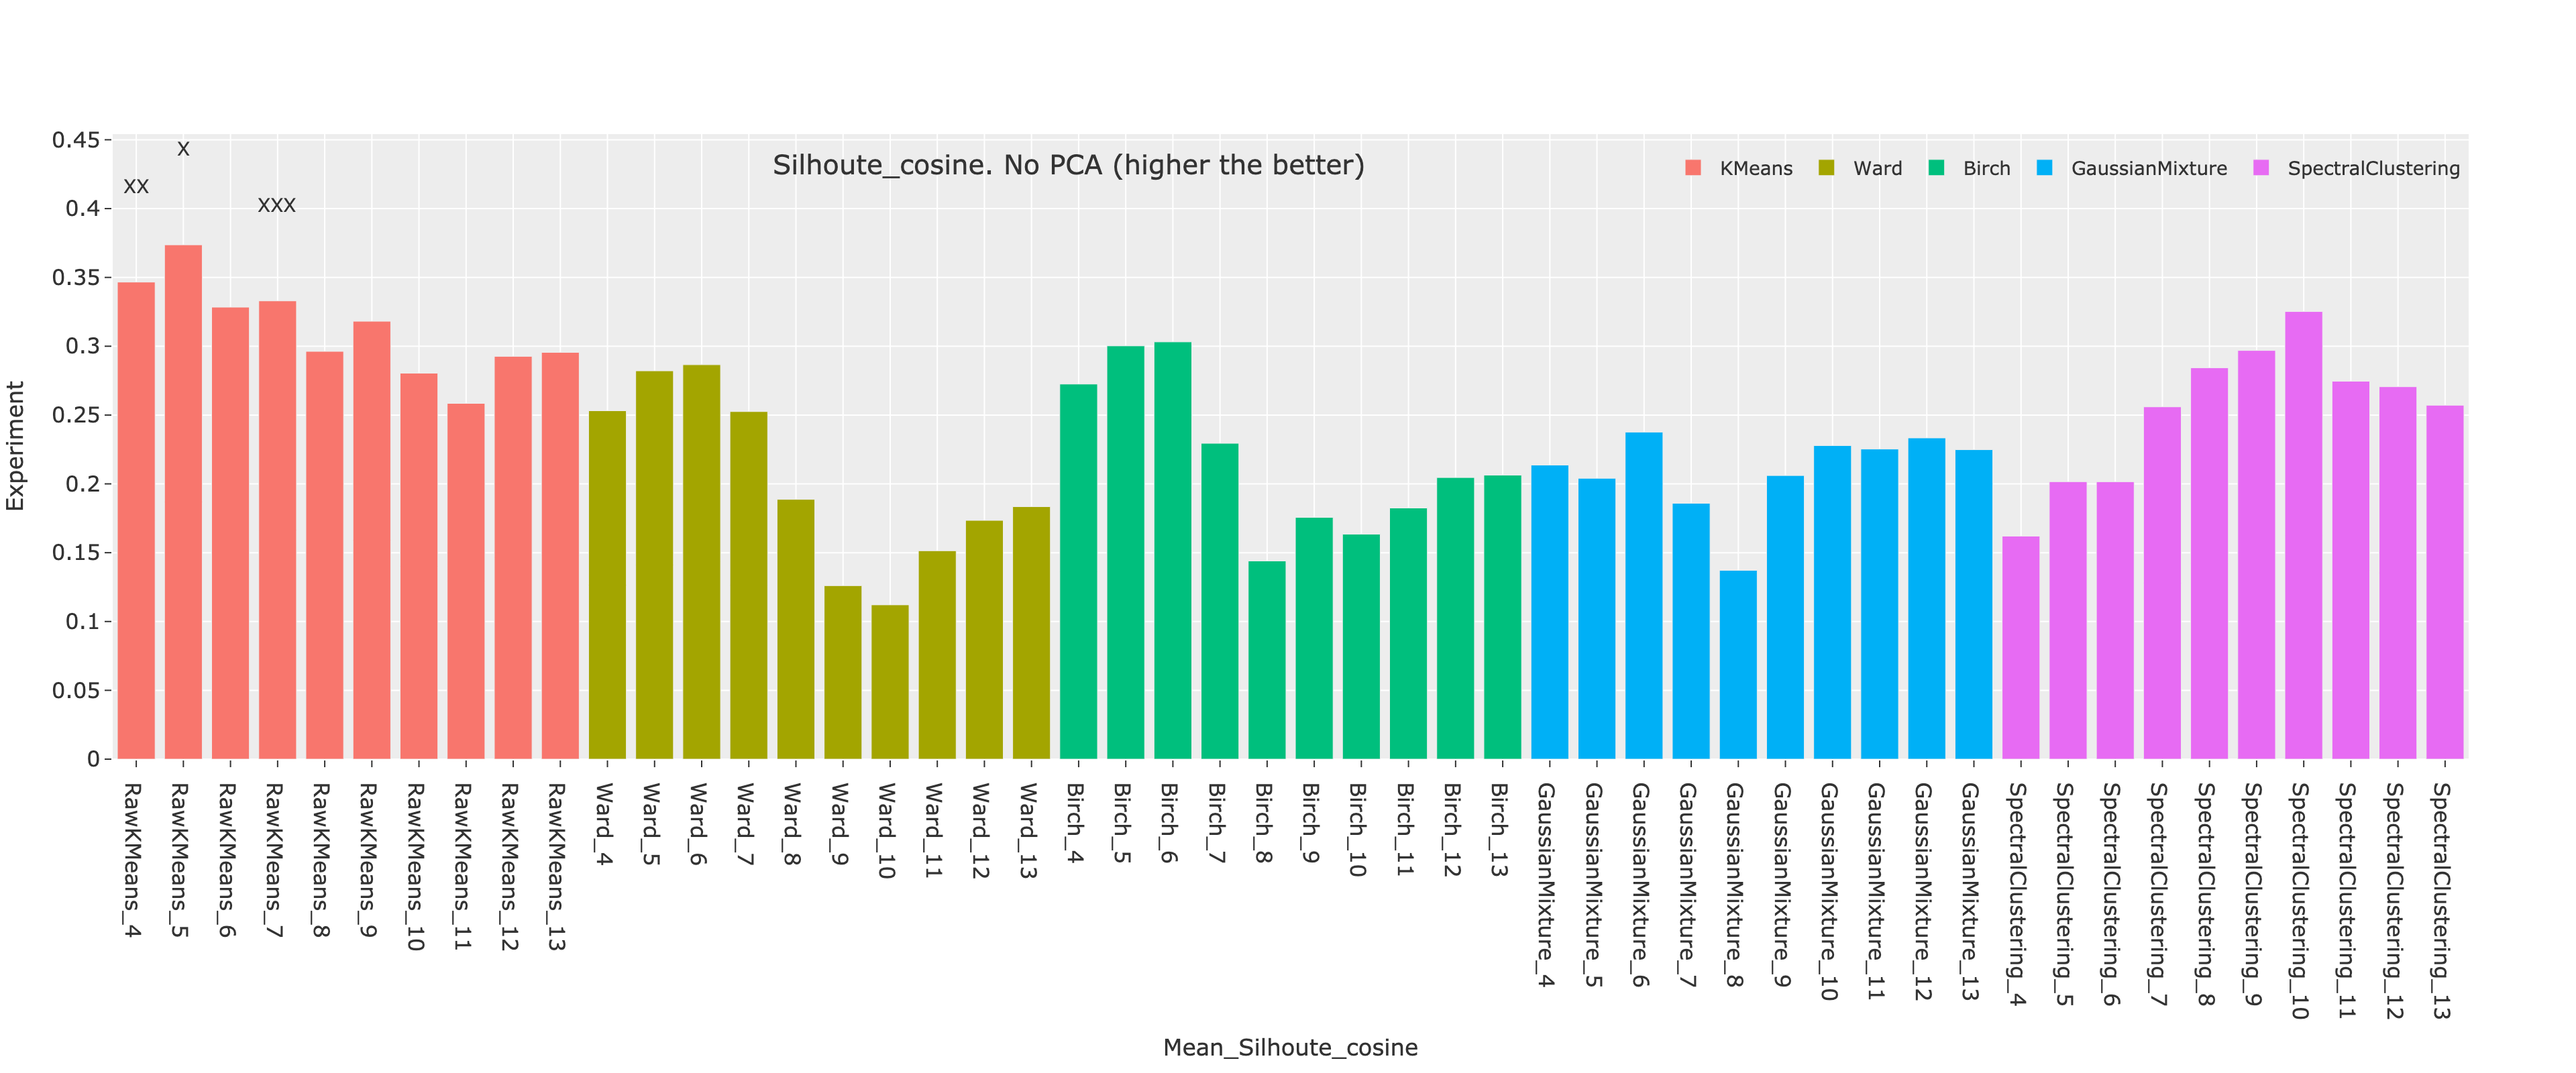
\includegraphics[width=\textwidth]{Sections/ClusteringAnalysis/Resources/cs_top3/PCA_top3_Silhoute_cosine.png}
        \caption{Silhouette using cosine distance}
        \label{fig:cs:cosine}
    \end{subfigure}
    \centering
    \begin{subfigure}[!t]{0.85\textwidth}
        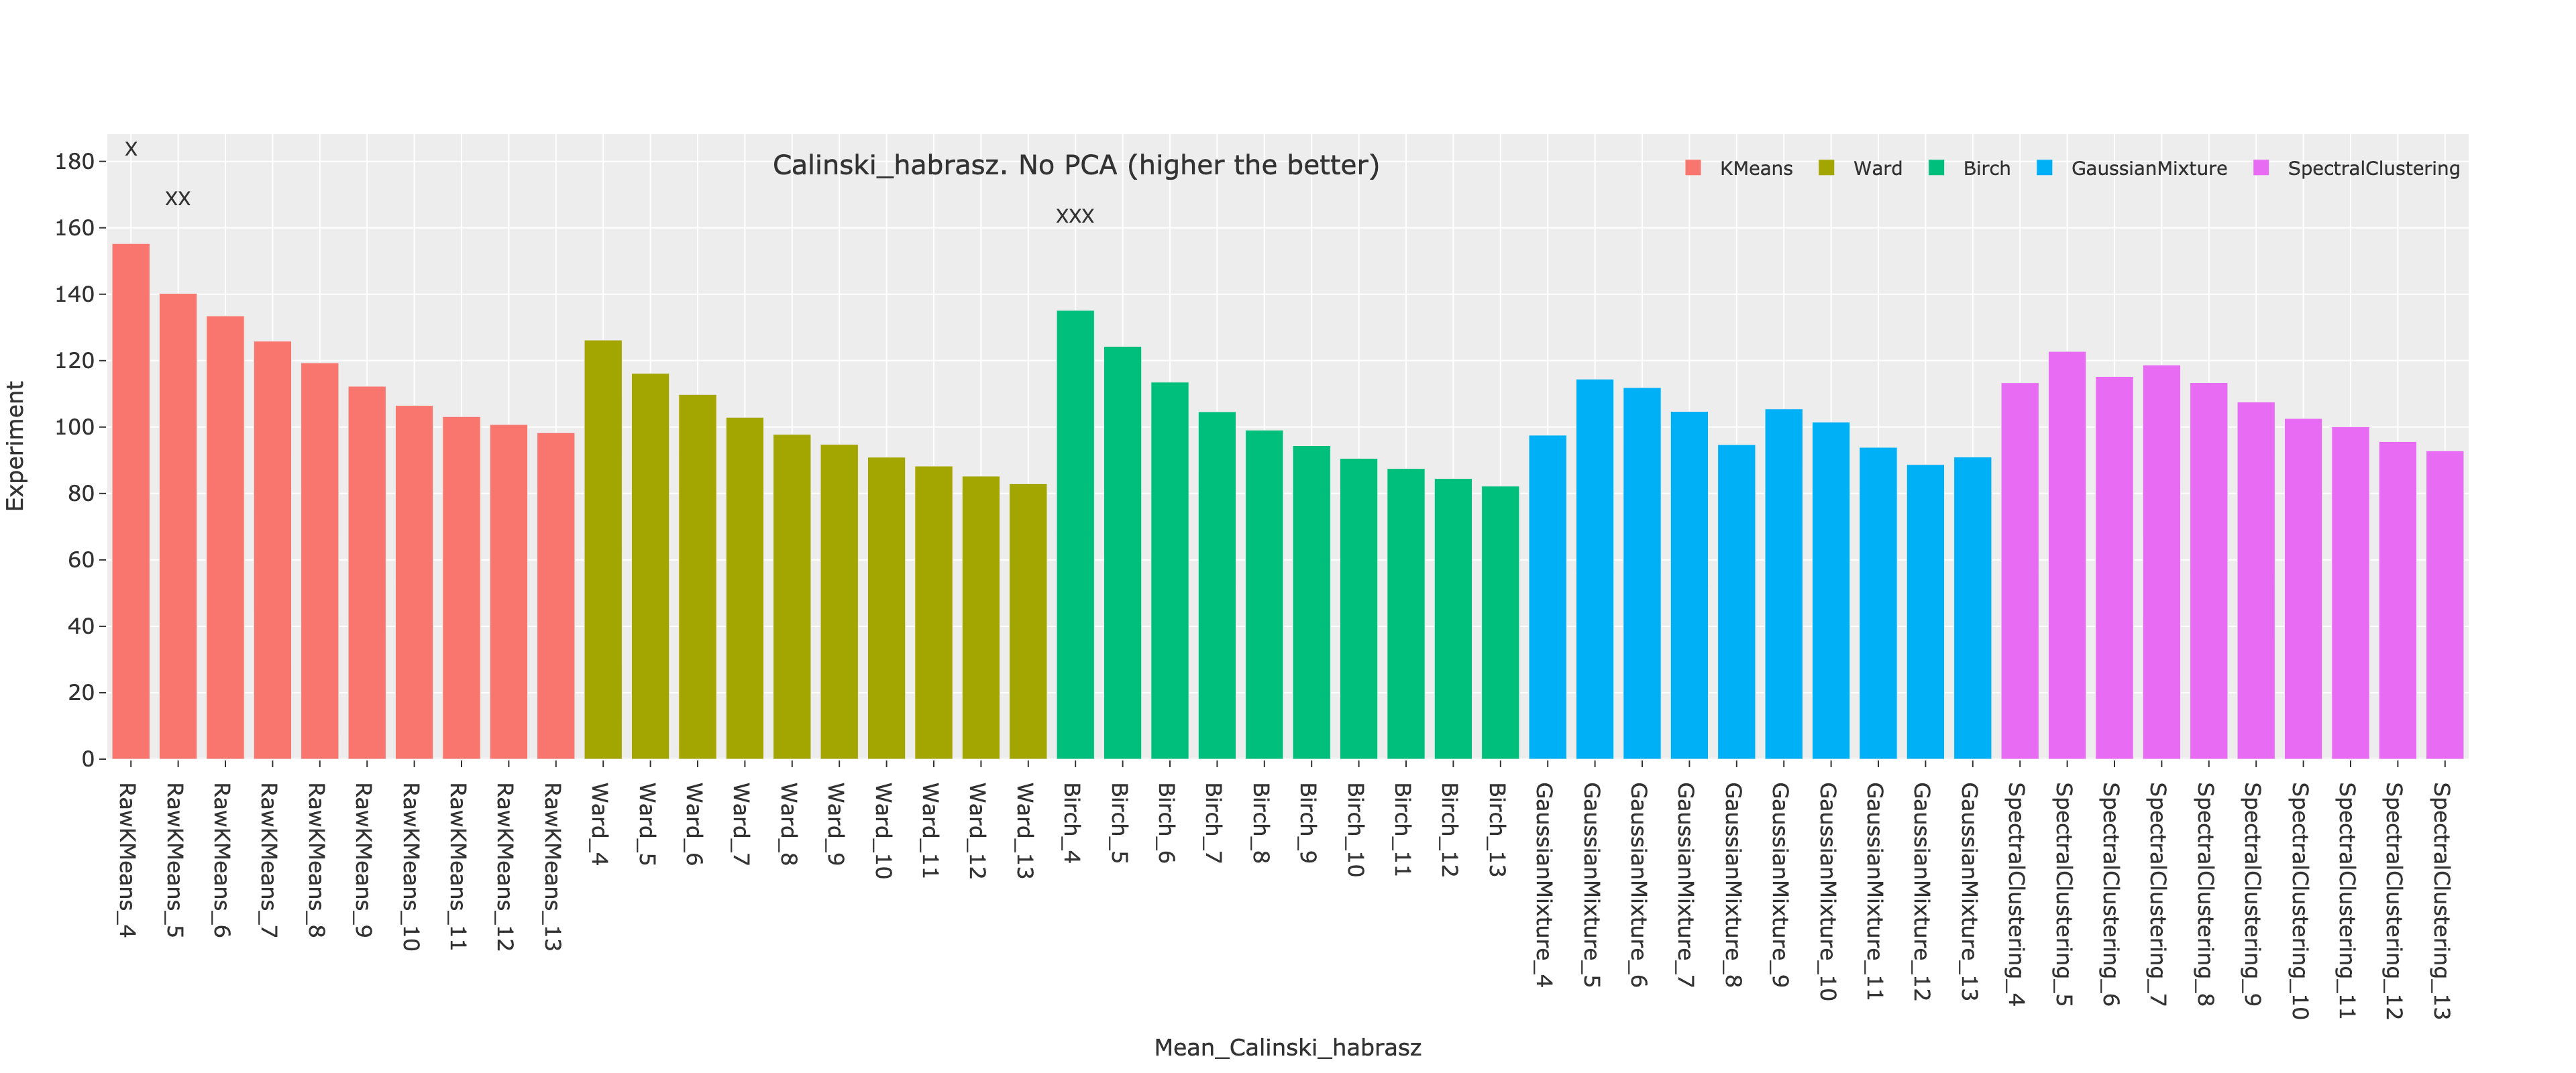
\includegraphics[width=\textwidth]{Sections/ClusteringAnalysis/Resources/cs_top3/PCA_top3_Calinski_habrasz.png}
        \caption{Calinski Harabasz}
        \label{fig:cs:cal_hab}
    \end{subfigure}
    \centering
    \begin{subfigure}[!t]{0.85\textwidth}
        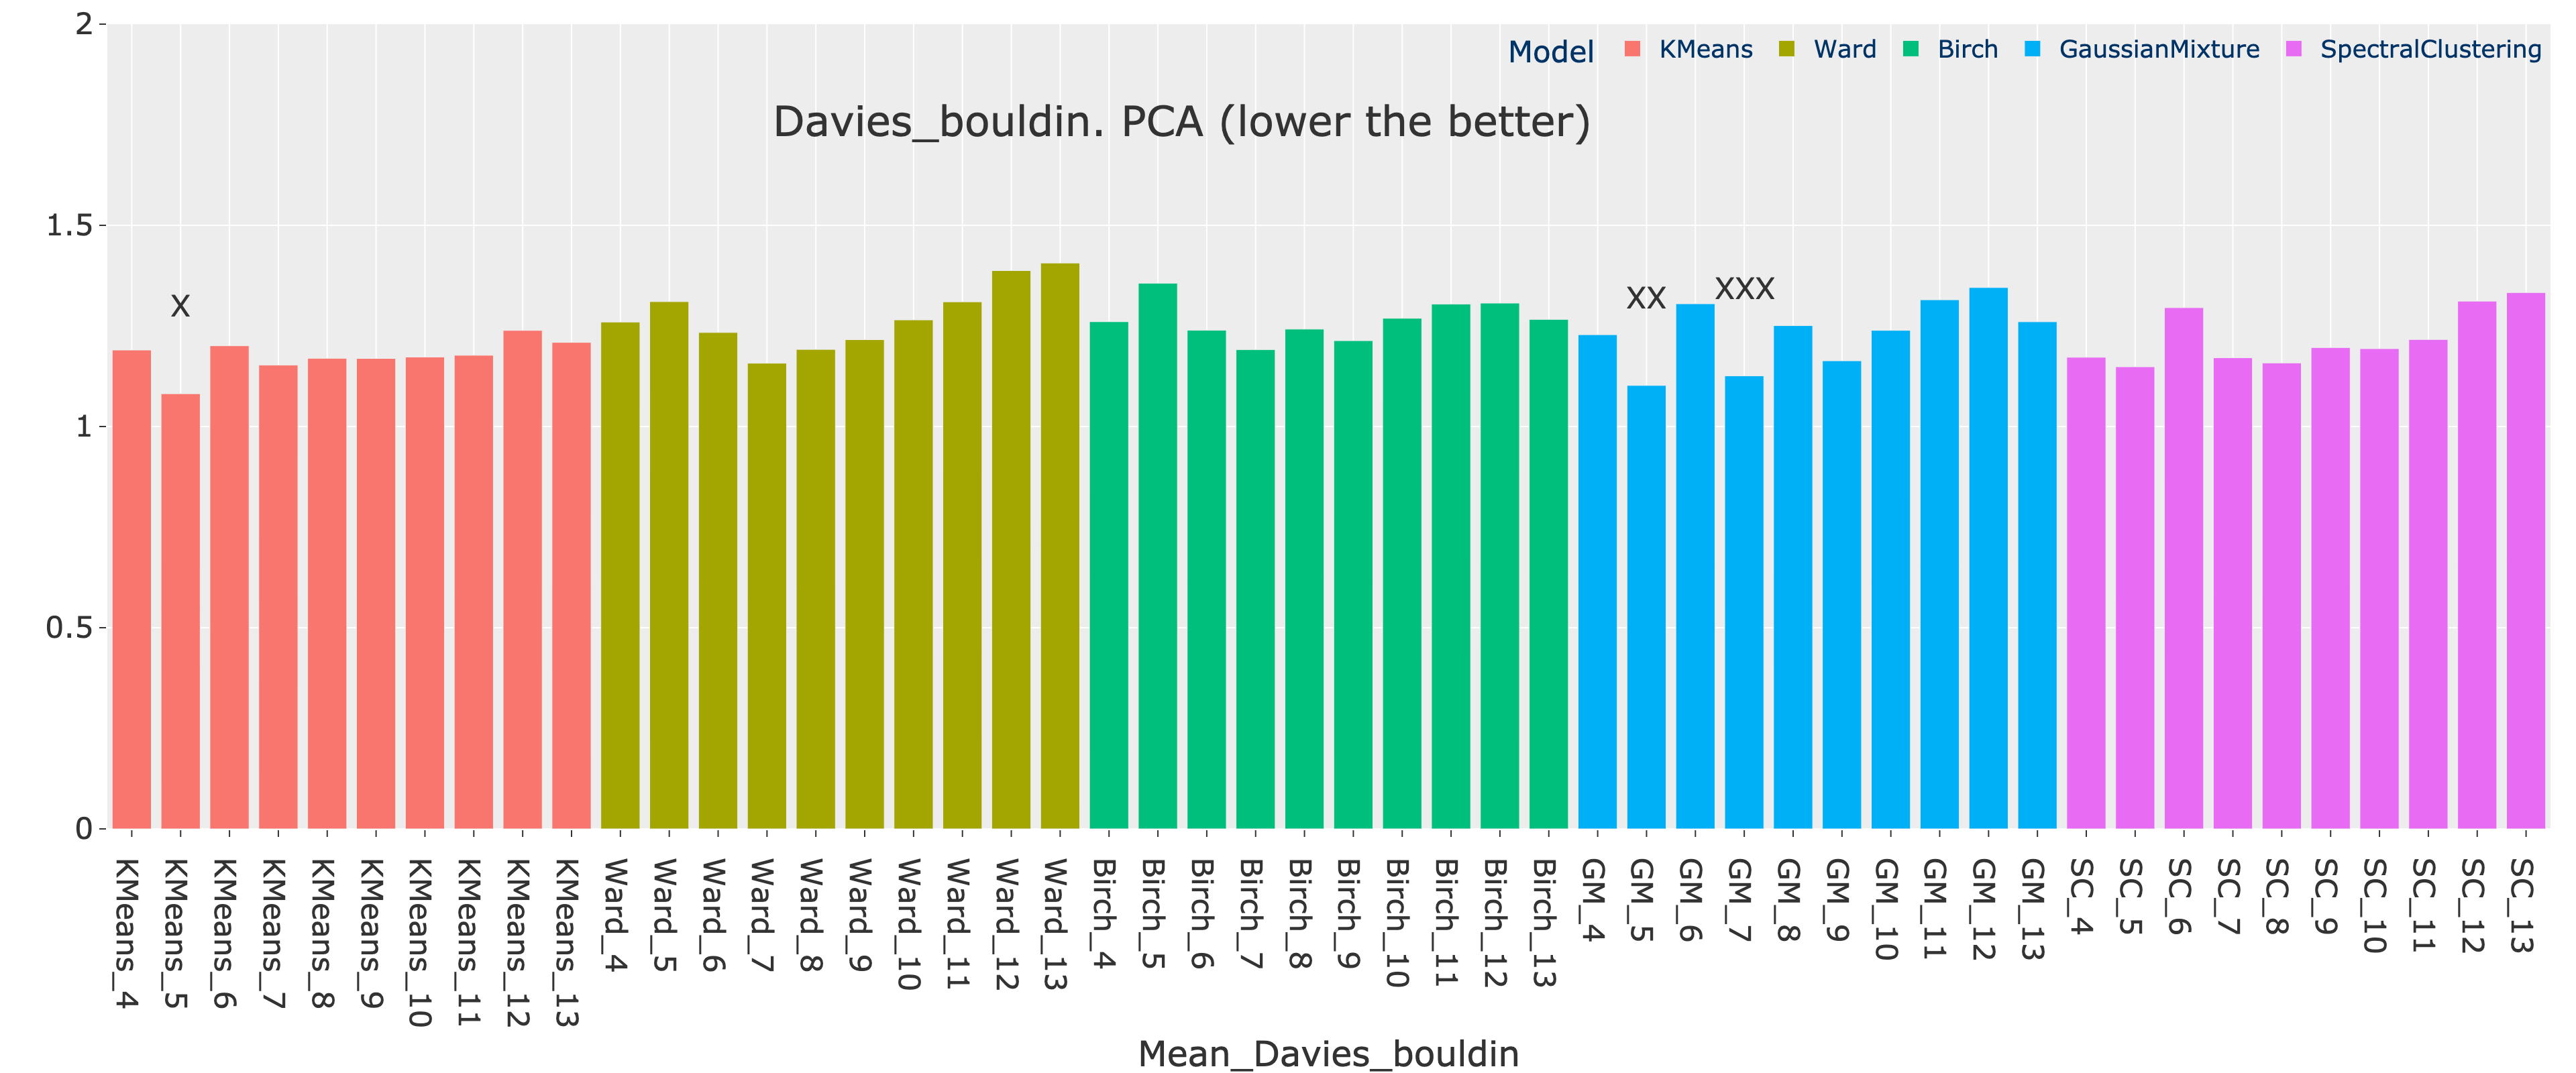
\includegraphics[width=\textwidth]{Sections/ClusteringAnalysis/Resources/cs_top3/PCA_top3_Davies_bouldin.png}
        \caption{Davies Bouldin}
        \label{fig:cs:dav_boul}
    \end{subfigure}
    \caption{The means of the three cluster metrics introduced in \cref{s:lit:clustering_metrics}: Silhouette (cosine), Calinski Harabasz and Davies Bouldin. Each of them asses different aspects of clustering and are used to determined the right clustering model for the MIBC cohort from TCGA. The gene expression is processed according to \cref{s:cs:methods} and PCA with 5 components was applied. For each metric the top 3 most performing models are marked by "X". }
    \label{fig:cs:cs_metrics}
\end{figure}


The performance of the five clustering methods across $K\in(4, 13)$ is displayed in
\cref{fig:cs:cs_metrics}; note lower bound of $K=4$ was chosen as lower K scored better than the others. The number of 'X' markers on top of the bar marks the model's position in top three. From the plots, it can be seen that the K-means generally performs the best across the clustering methods. A general trends across the methods is that their inverse relationship between the algorithm's performance over the number of groups. This is the most evident in the Calinski Harabasz score (\cref{fig:cs:cal_hab}) and in Davies Bouldin index (\cref{fig:cs:dav_boul}), but less pronounced in the Silhouette score (\cref{fig:cs:cosine})


\begin{figure}[!htb]
    \captionsetup[subfigure]{justification=Centering}
    \centering
    \begin{subfigure}[!t]{0.49\textwidth}
        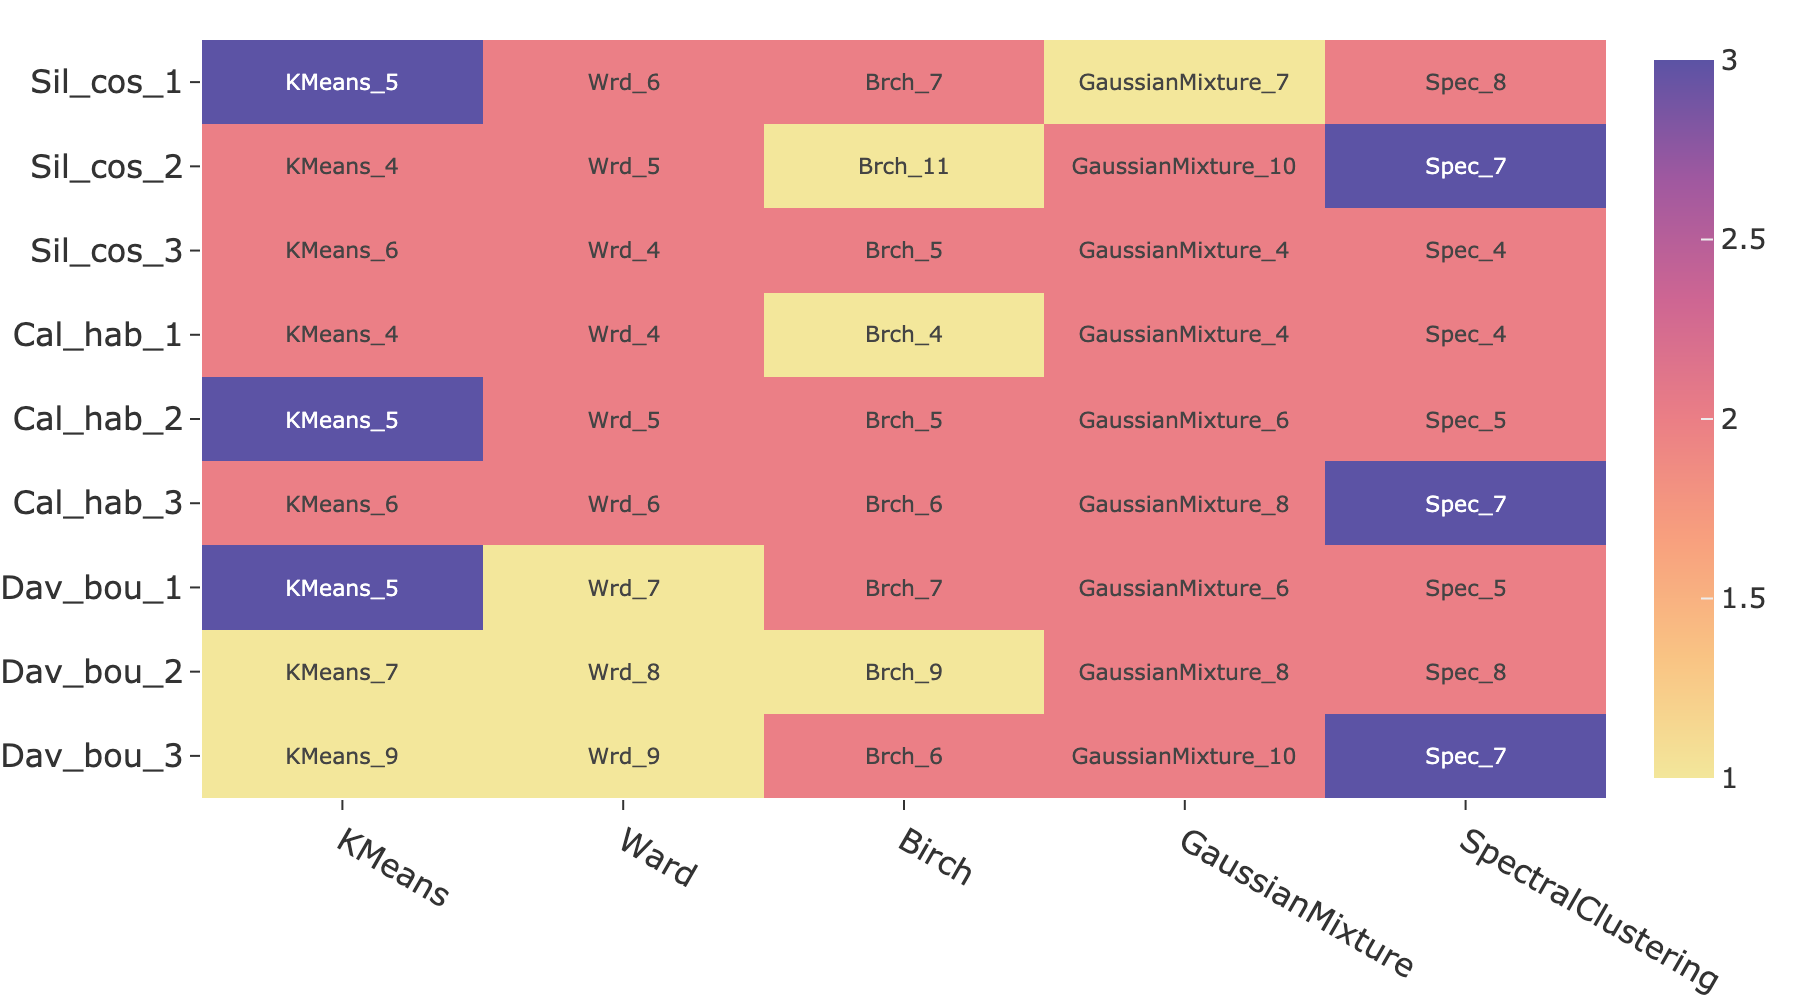
\includegraphics[width=\textwidth]{Sections/ClusteringAnalysis/Resources/cs_top3/top3_cs_gen_top3_heatmap_pca.png}
        \caption{Most frequent cluster model}
        \label{fig:cs:heatmap_gen}
    \end{subfigure}
    \centering
    \begin{subfigure}[!t]{0.49\textwidth}
        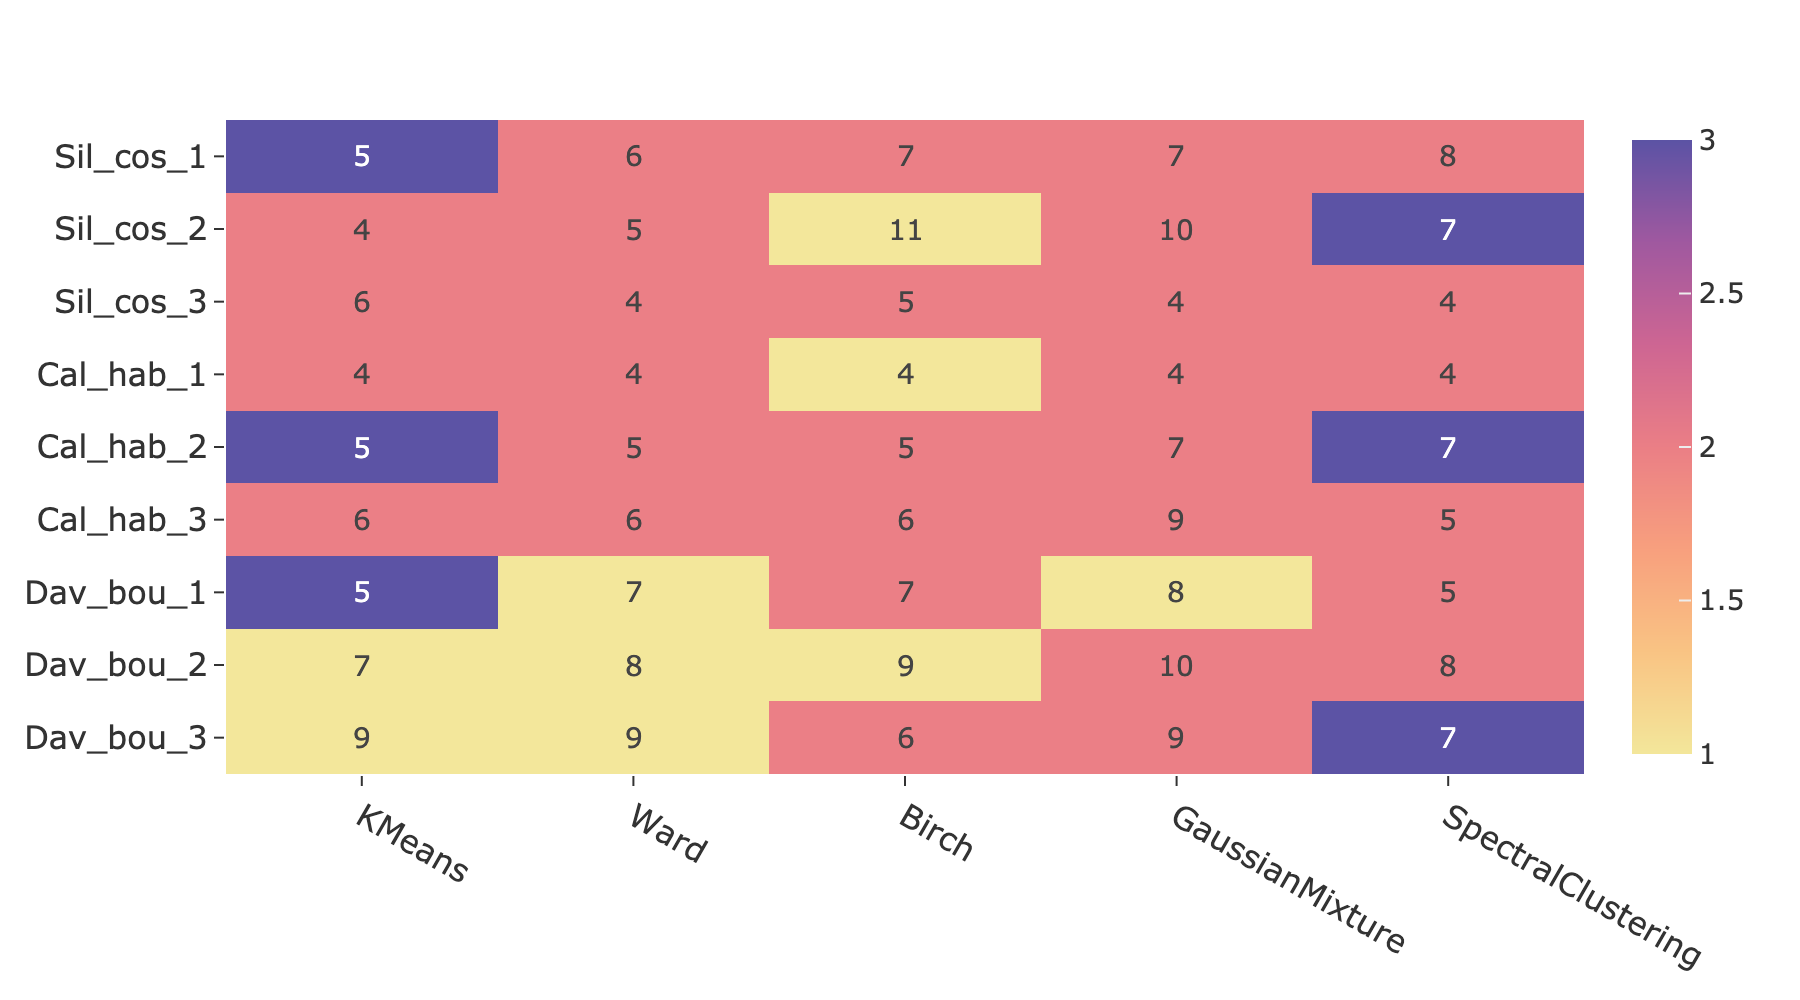
\includegraphics[width=\textwidth]{Sections/ClusteringAnalysis/Resources/cs_top3/top3_cs_size_top3_heatmap_pca.png}
        \caption{Most frequent K in top 3}
        \label{fig:cs:heatmap_cs}
    \end{subfigure}
    \caption{Most frequent model and K by the clustering metrics. For each heatmap the rows are given by top model/K for that metric, while the X axis contains the methods used. The colouring is done per column, so it can be determine the right configuration per model and for the number of clusters.}
    \label{fig:cs:cs_metrics_heatmap}
\end{figure}

To aid the decision making, the top 3 most performing configuration is displayed per cluster metric in \cref{fig:cs:cs_metrics_heatmap}. The two heat-maps are similar, each column represents the algorithm while the rows the cluster metrics, the colouring is done by the occurrence per algorithm. In the first heatmap, \cref{fig:cs:heatmap_gen} the colour is proportional with the occurrence of the model configuration, while in the second \cref{fig:cs:heatmap_cs} the colouring is given by the number of clusters. This means, that the first plot gives the most popular model configuration per algorithm, while the second the most frequent K. From this, K-Means with 5, Spectral Clustering with 7 clusters and K=5 and K=7 are the most frequent methods/group sizes. 


\paragraph*{Silhouette distribution}

% Sillhouette
So far the decision making was made by using the mean of the clustering metrics, while this helped to select the model and the number of clusters, the average does not contain the variation in the scores. To address, the distribution of the Silhouette scores\footnote{The experiment for this is an adapted version of the \href{https://tinyurl.com/sillhouete-distrib}{example} from Scikit-learn library.} was plotted in \cref{fig:cs:sill_distrib} for the K-means model between 3 to 6 clusters. A restricted range of K was used to facilitate the visualisation and the previous results (\cref{fig:cs:cs_metrics}) suggests that there is little benefit for adding more. 


\begin{figure}[!t]
    \captionsetup[subfigure]{justification=Centering}
    \centering
    \begin{subfigure}[!t]{0.49\textwidth}
        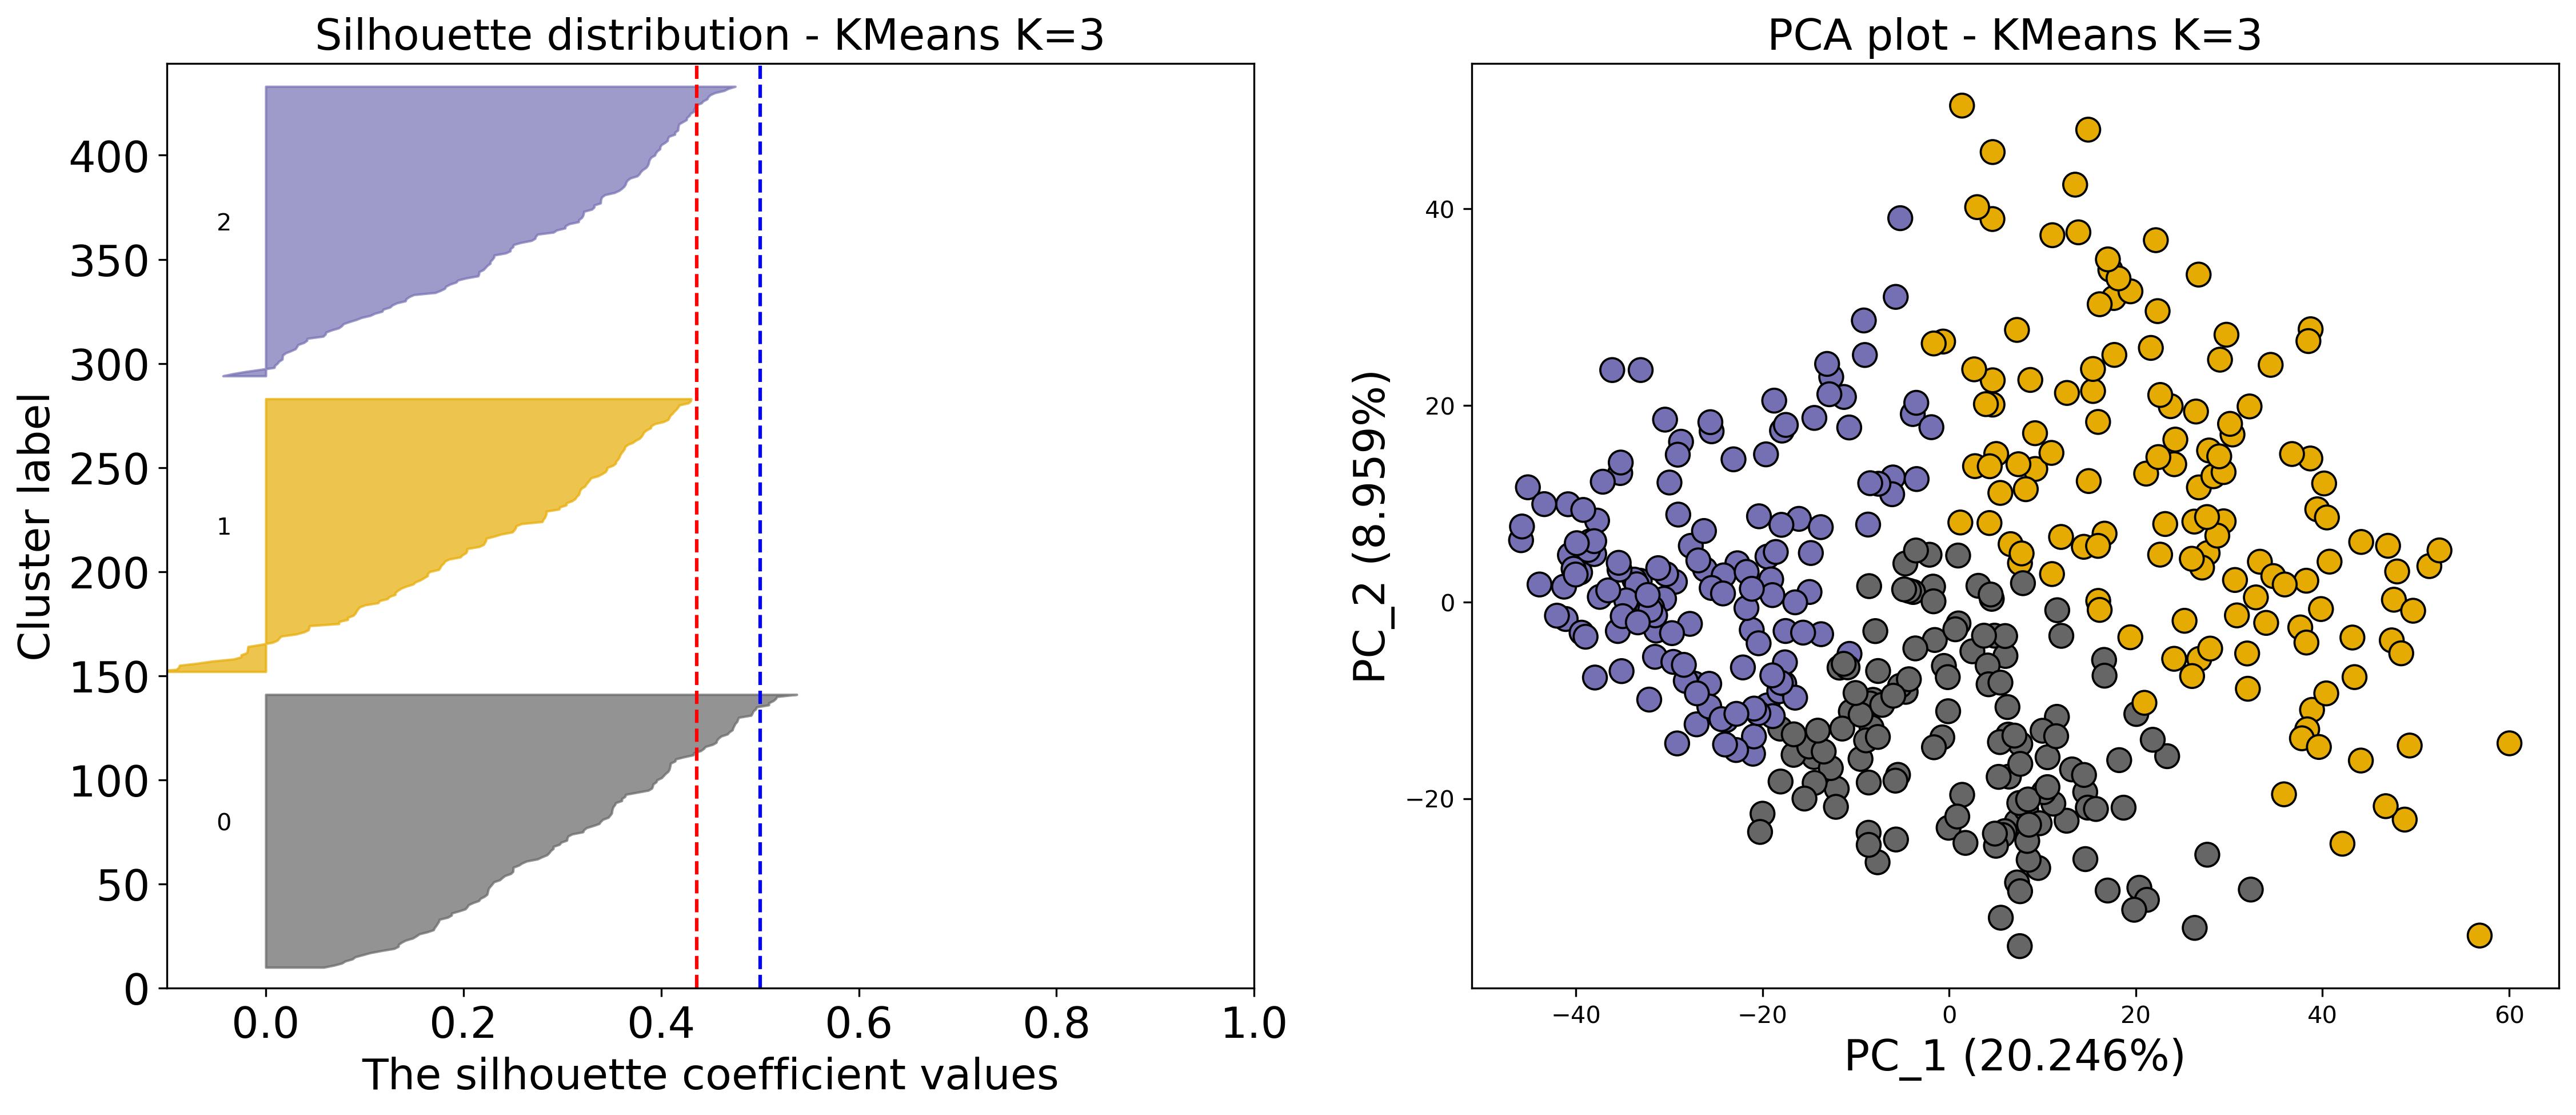
\includegraphics[width=\textwidth]{Sections/ClusteringAnalysis/Resources/cs_top3/sill_distrib/KMeans_3_sill_distrib.png}
        \caption{K=3}
    \end{subfigure}
    \centering
    \begin{subfigure}[!t]{0.49\textwidth}
        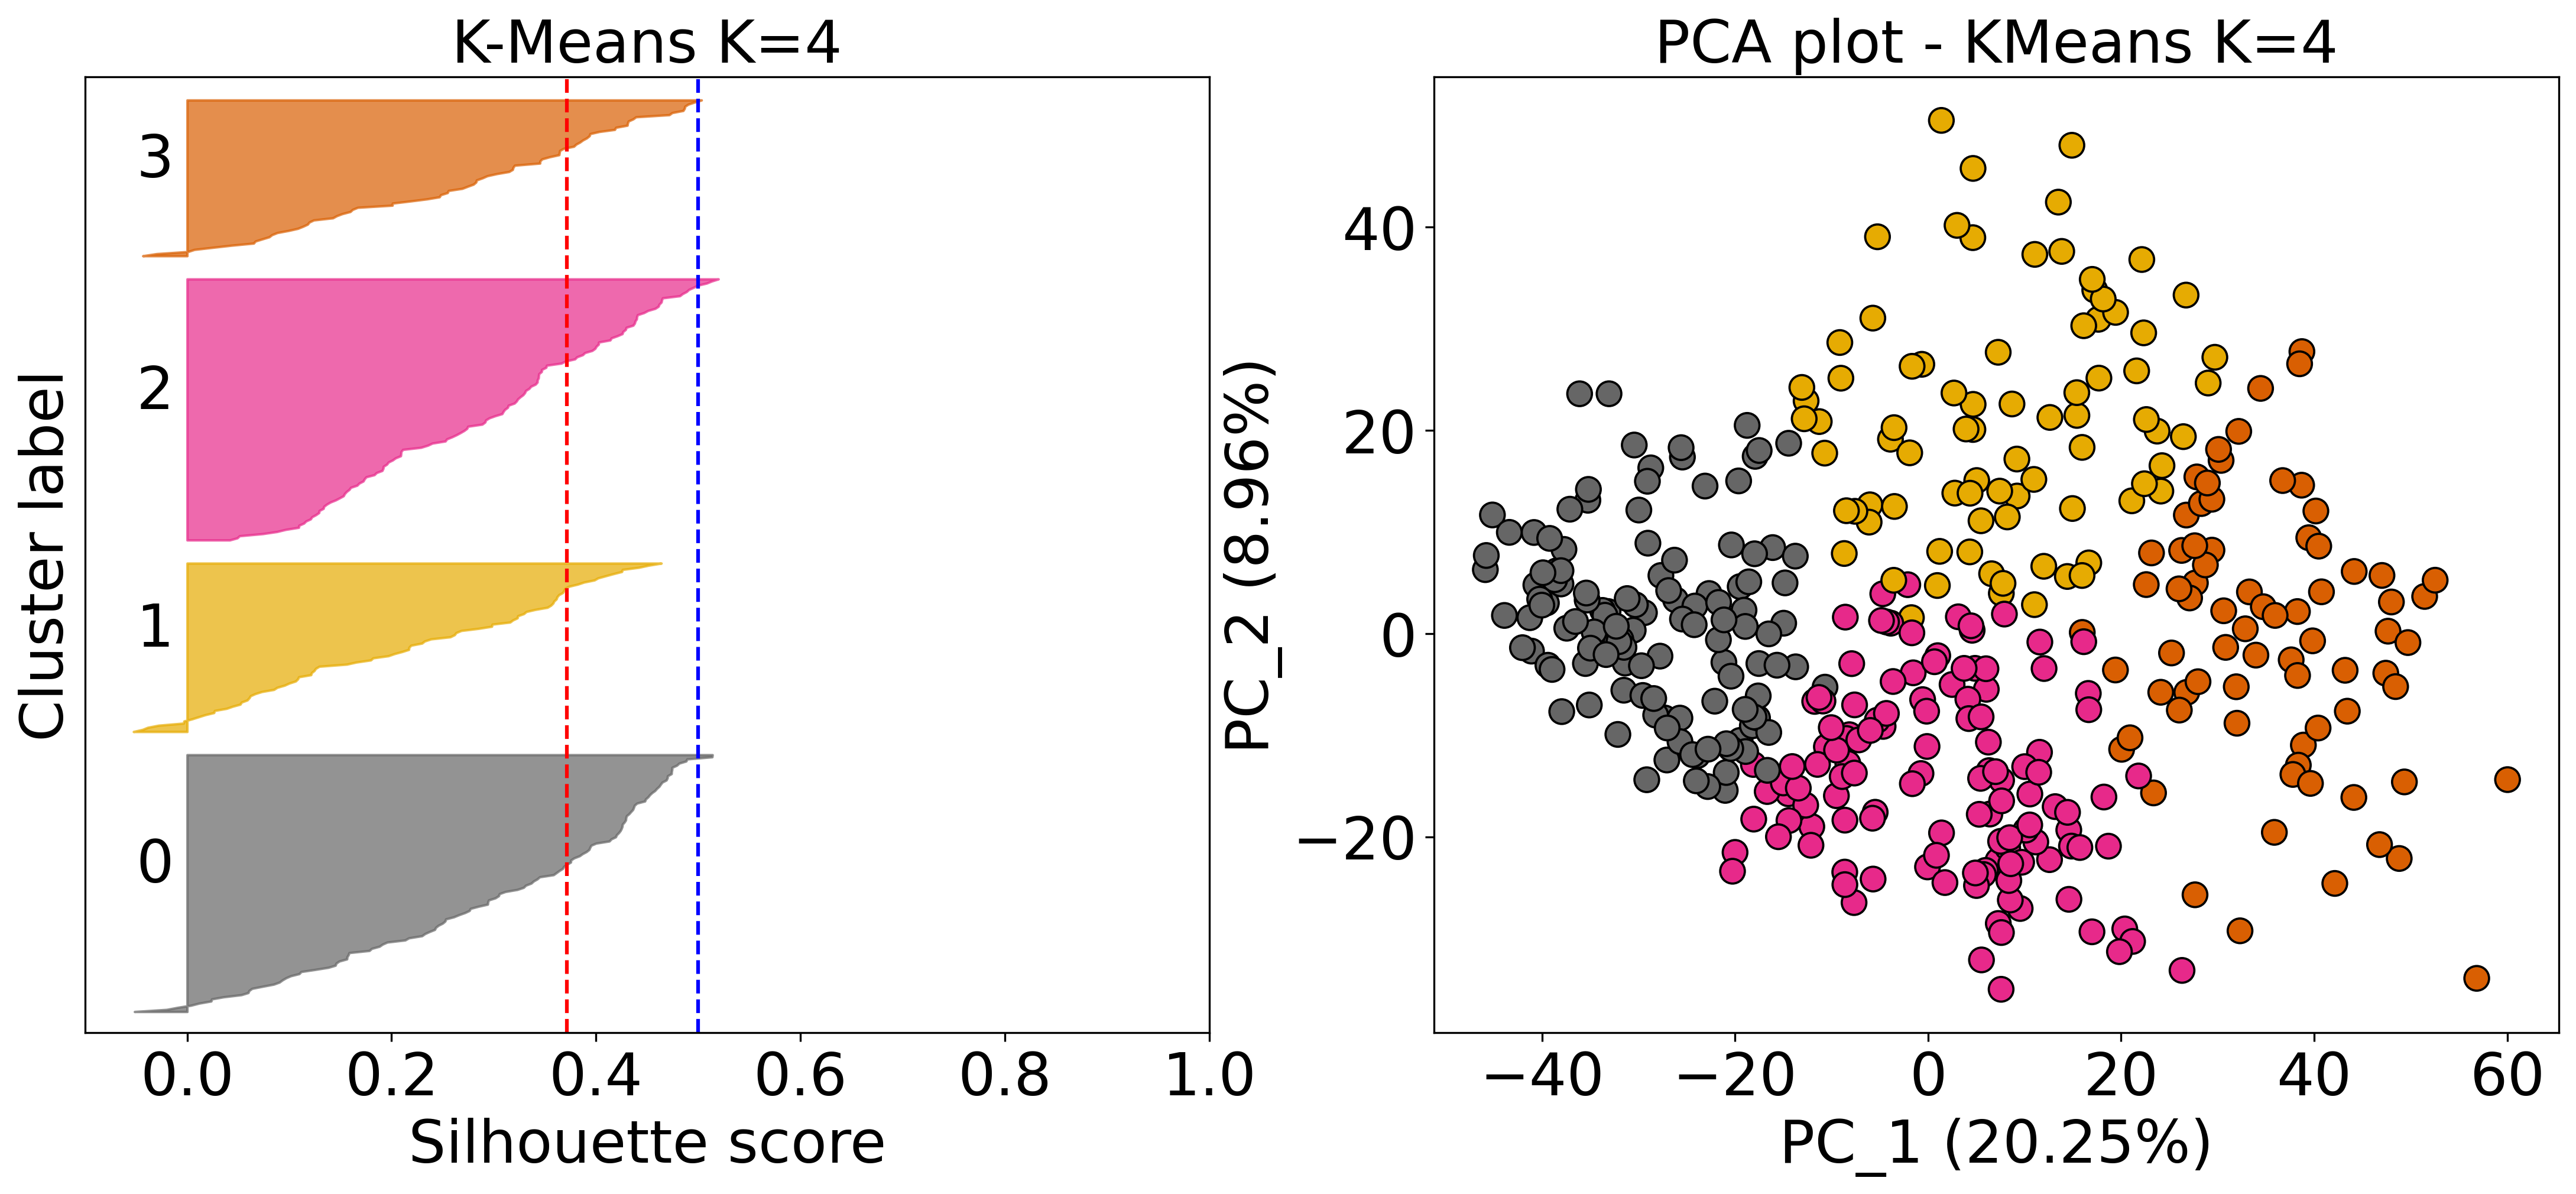
\includegraphics[width=\textwidth]{Sections/ClusteringAnalysis/Resources/cs_top3/sill_distrib/KMeans_4_sill_distrib.png}
        \caption{K=4}
    \end{subfigure}
    \centering
    \begin{subfigure}[!t]{0.49\textwidth}
        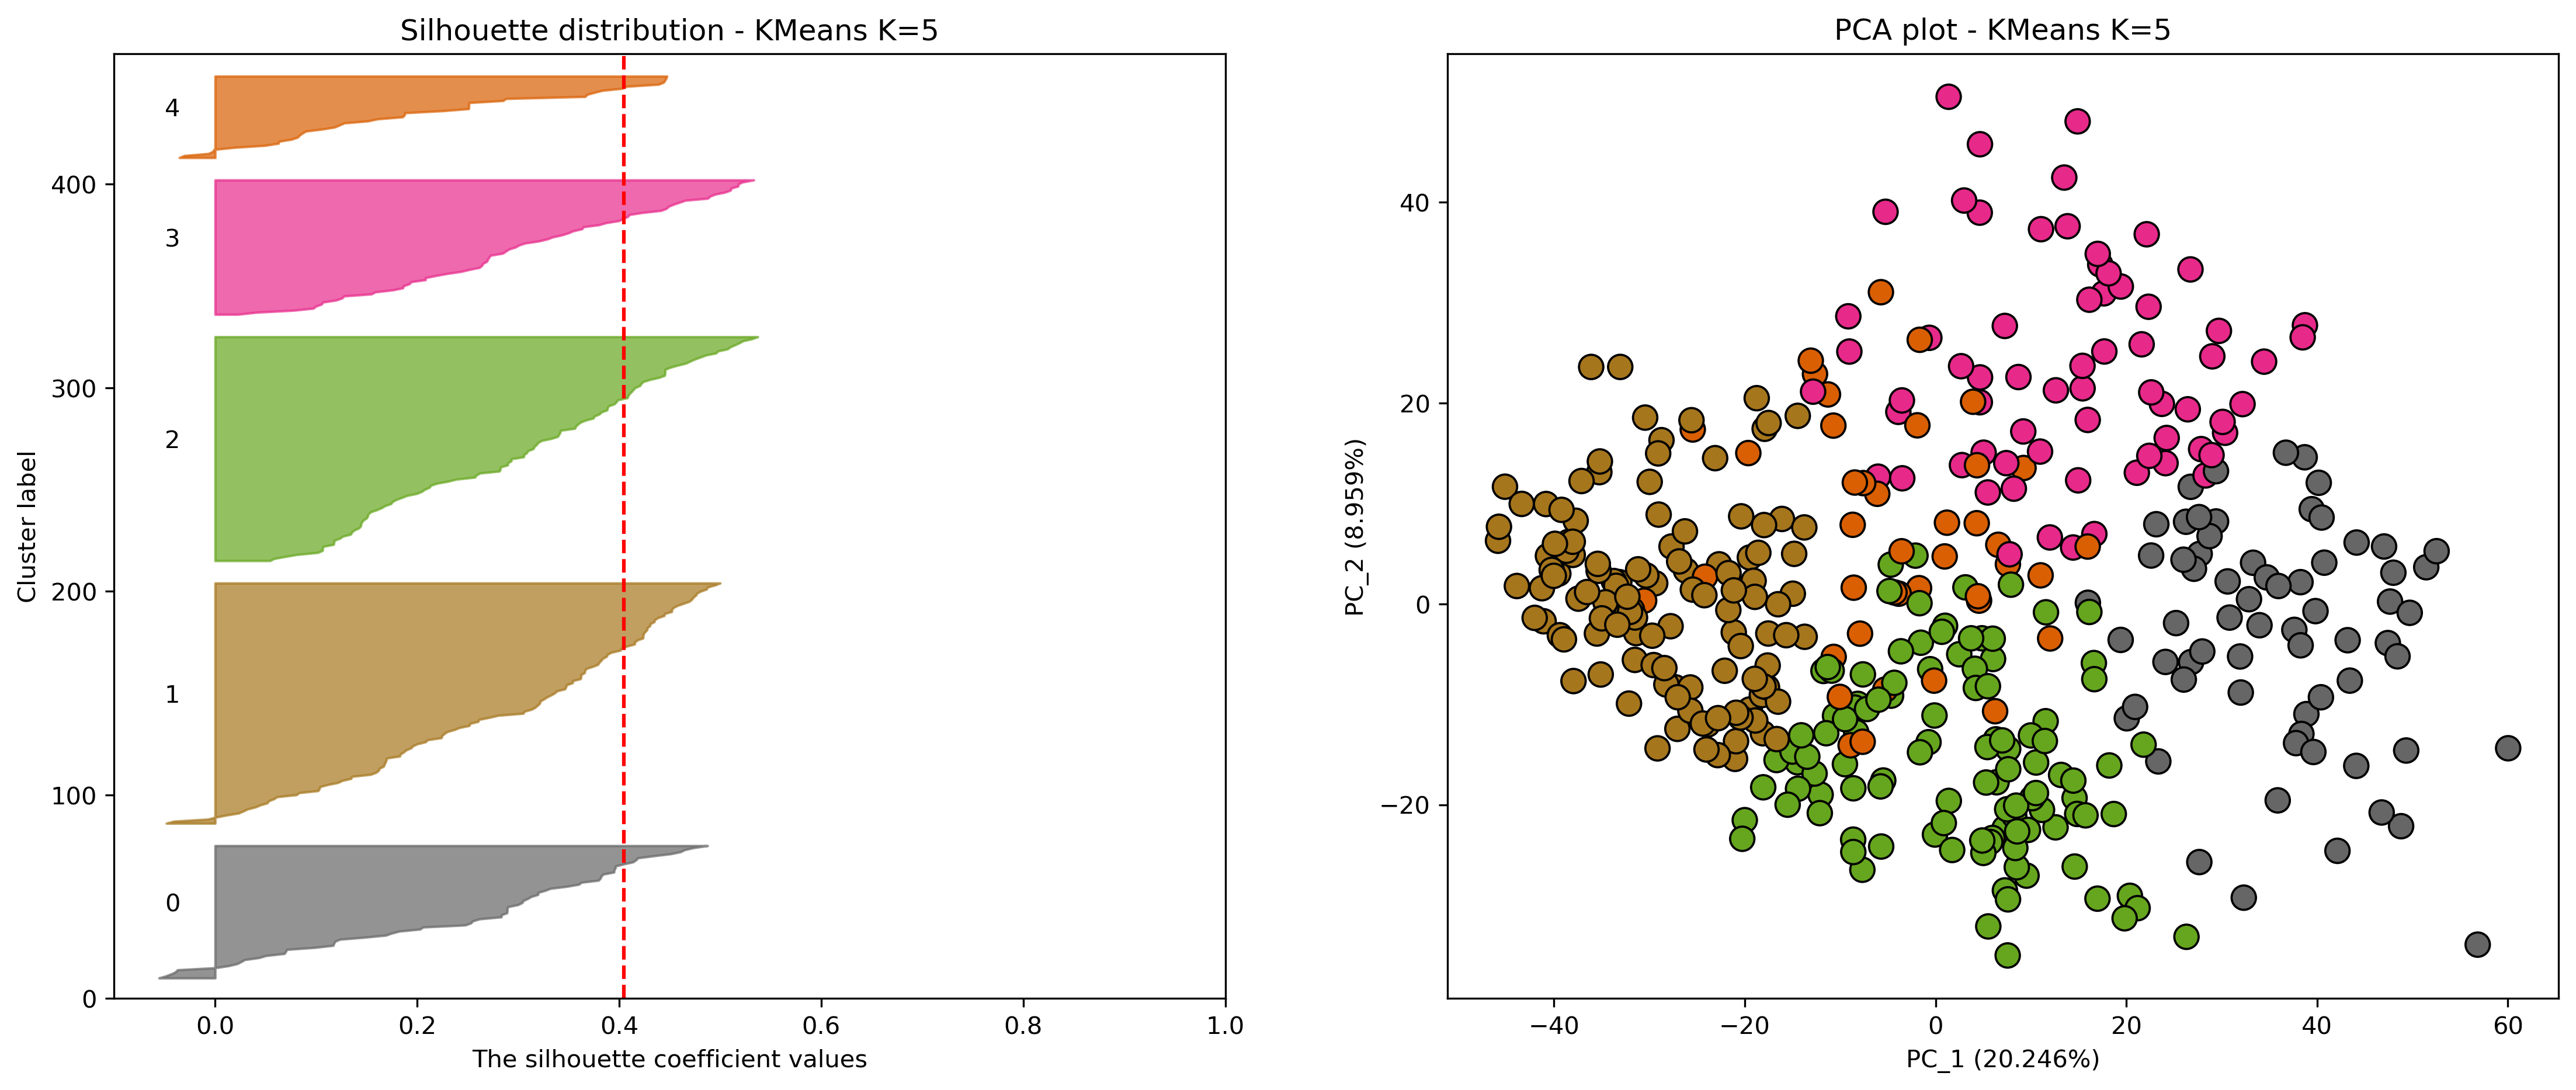
\includegraphics[width=\textwidth]{Sections/ClusteringAnalysis/Resources/cs_top3/sill_distrib/KMeans_5_sill_distrib.png}
        \caption{K=5}
    \end{subfigure}
    \centering
    \begin{subfigure}[!t]{0.49\textwidth}
        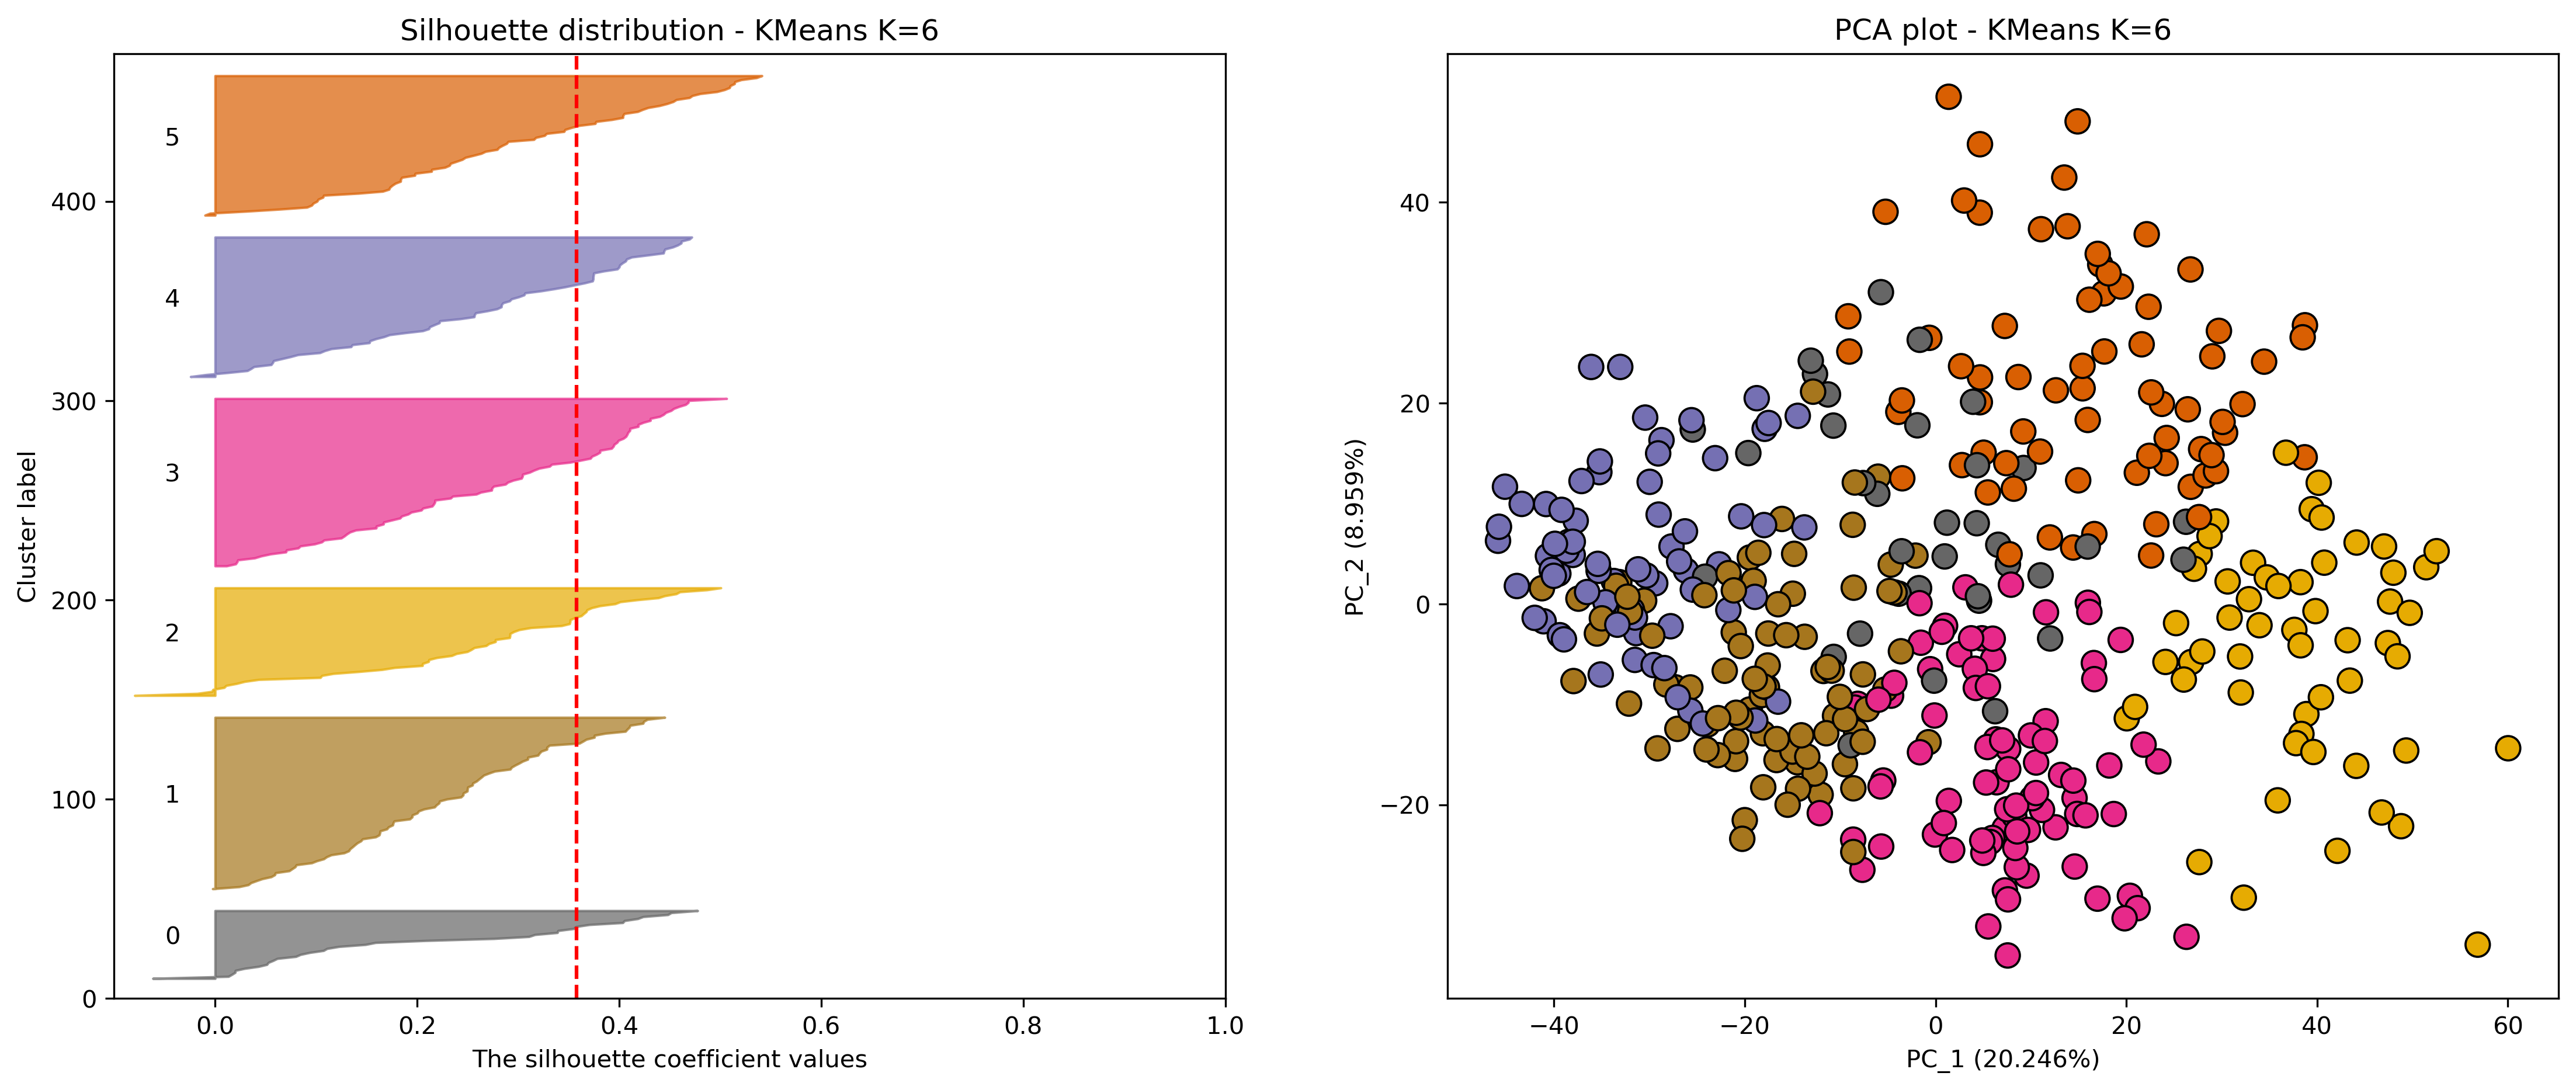
\includegraphics[width=\textwidth]{Sections/ClusteringAnalysis/Resources/cs_top3/sill_distrib/KMeans_6_sill_distrib.png}
        \caption{K=6}
    \end{subfigure}
    \centering
    \begin{subfigure}[!t]{0.49\textwidth}
        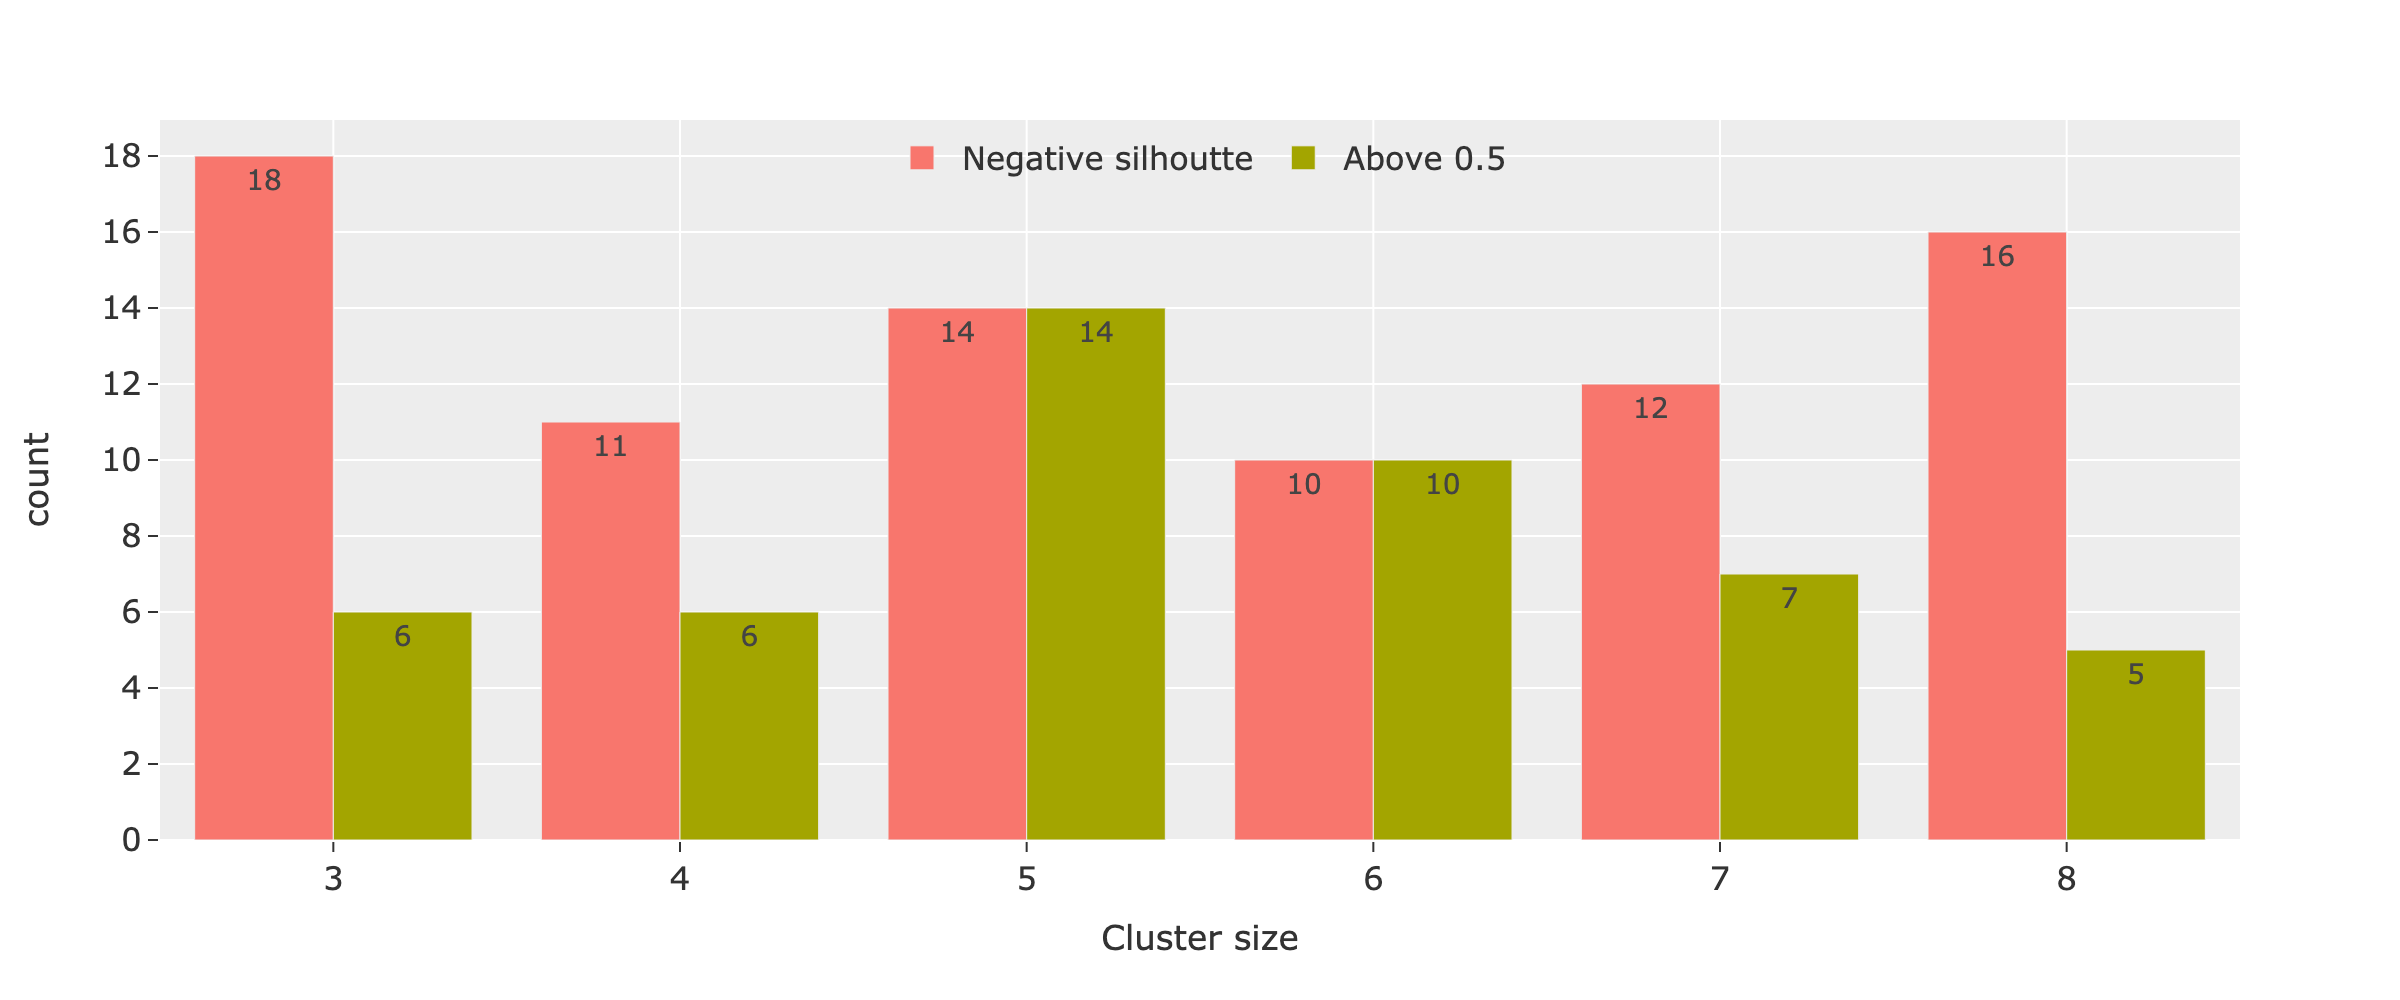
\includegraphics[width=\textwidth, keepaspectratio]{Sections/ClusteringAnalysis/Resources/cs_top3/sill_distrib/sill_neg_above_th.png}
        \caption{Number of samples with negative and above 0.5 Silhouette scores}
    \end{subfigure}
    \centering
     \begin{subfigure}[!t]{0.49\textwidth}
        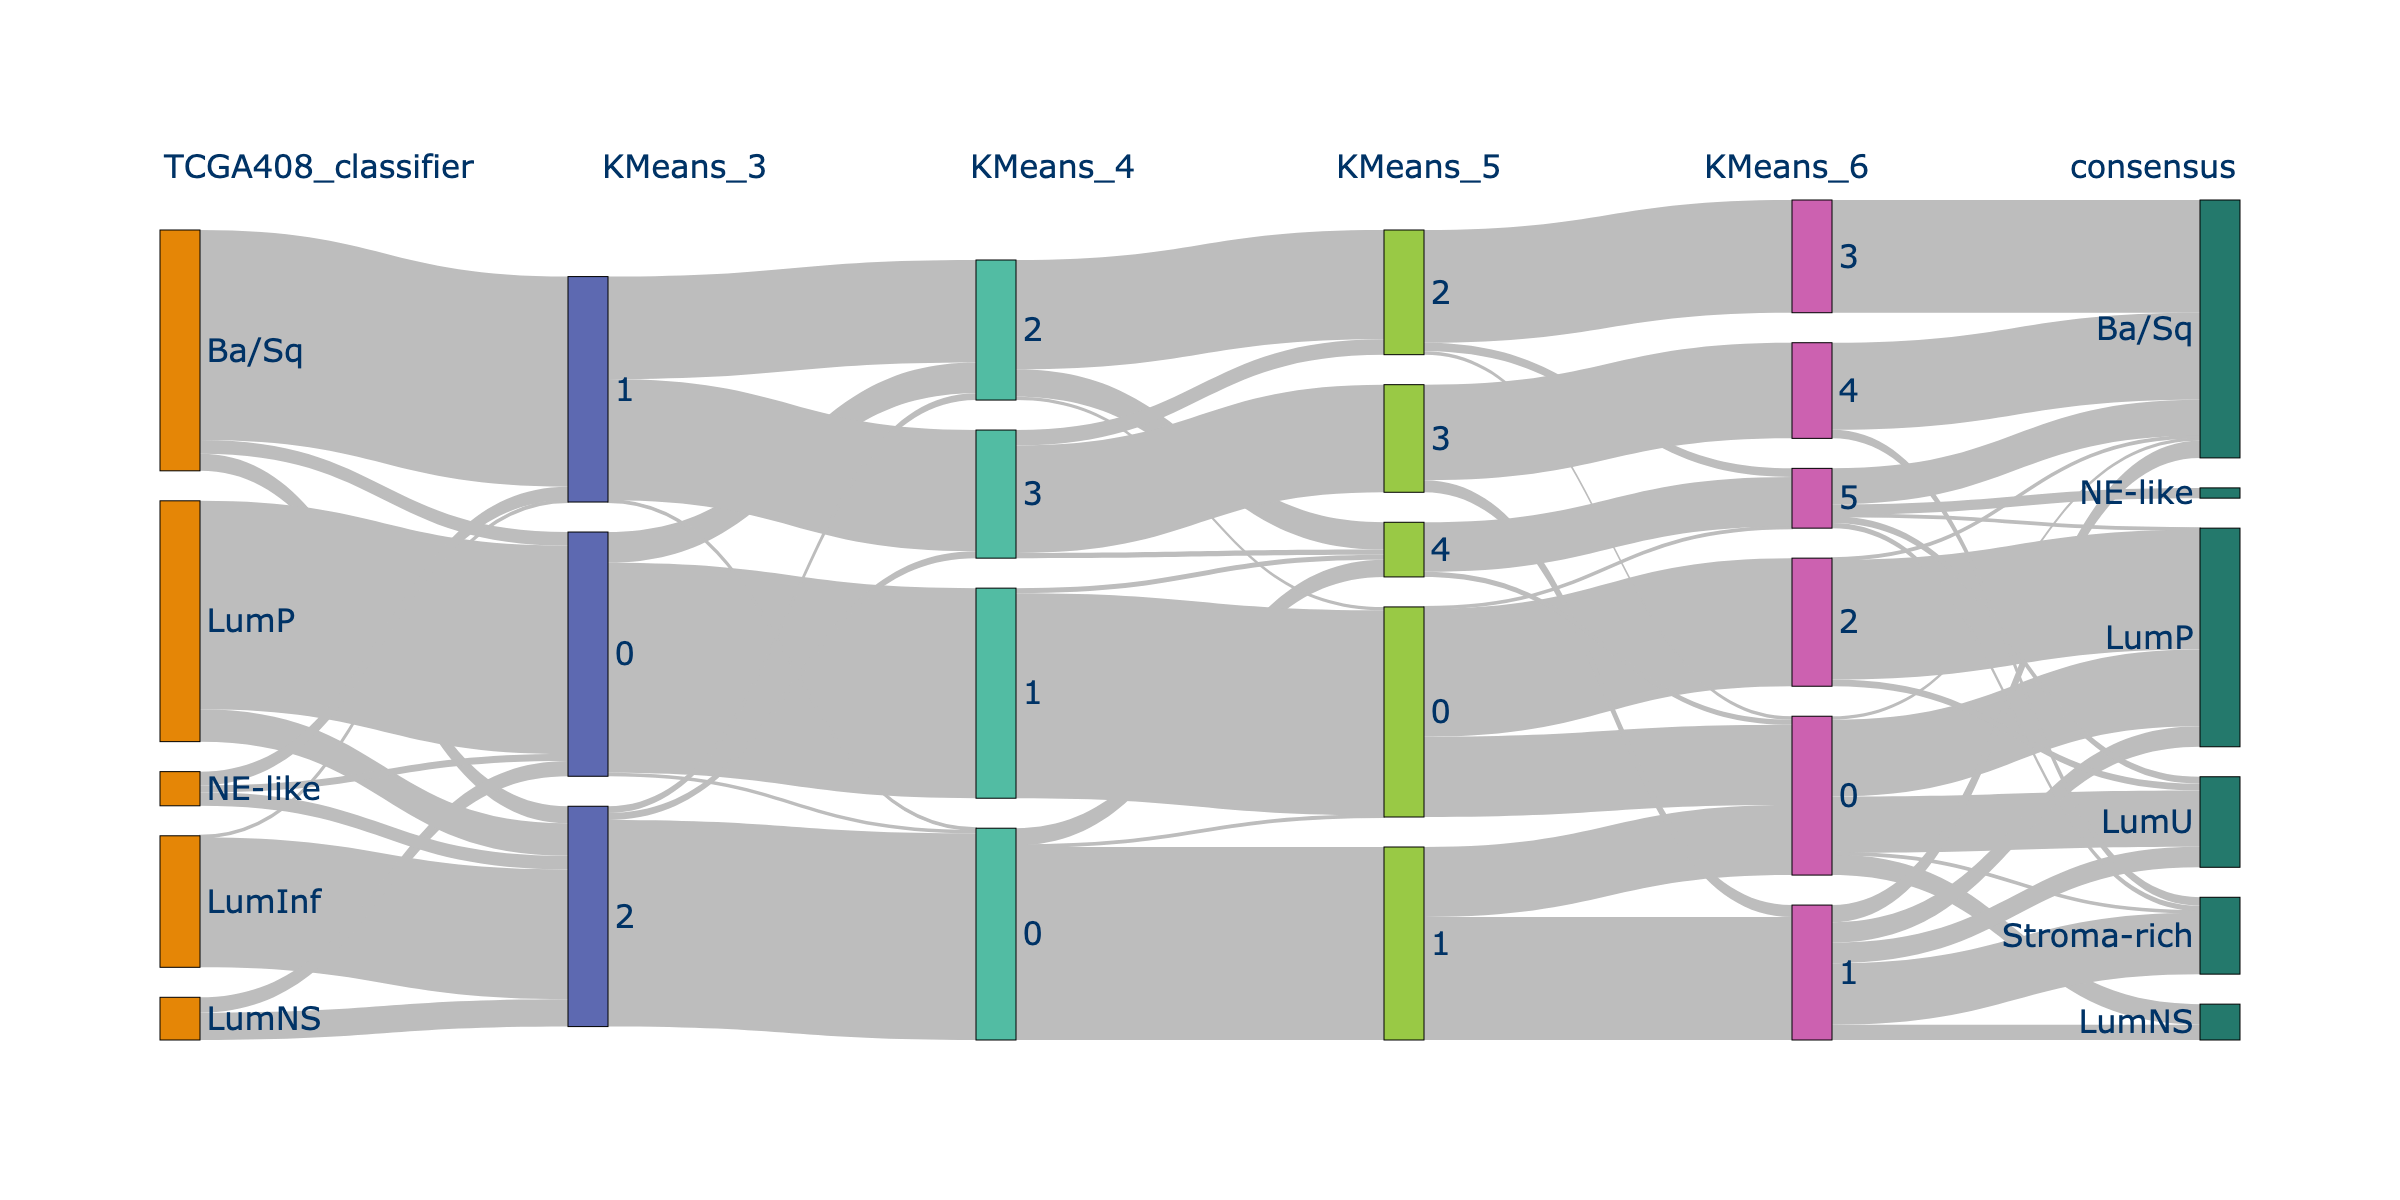
\includegraphics[width=\textwidth, keepaspectratio]{Sections/ClusteringAnalysis/Resources/cs_top3/sill_distrib/sky_kMeans.png}
        \caption{Comparison across clustering methods}
    \end{subfigure}
    \centering
    \caption{The silhouette distribution of the K-means model for K ranging from 3 to 6. The scatter plot on the right plots the first 2 components of PCA (4 components) coloured by the cluster labels from the method. A good silhouette score is considered to be above 0.5, which is marked on by the red dotted line. The sankey plot shows the comparison across the different configurations of K-Means.}
    \label{fig:cs:sill_distrib}
\end{figure}


The first two rows on \cref{fig:cs:sill_distrib} present the subplots containing the Silhouette distribution and the 2-d scatter plot of the first two principal components. Generally, a silhouette score above 0.5 is considered a good good and that the sample belongs to its group, values around 0 indicates that the sample can be grouped to multiple clusters, while the negative values denotes the miss-labelled of the samples. Across the top 4 plots, it can be seen that the vast majority of the samples are below the 0.5 threshold. This indicates the lack of clear defined clusters and high heterogeneity of the data which is a known aspect of the MIBC 'molecular profile' (see \cref{s:lit:bladder_cancer}). As it was mentioned before, K=3 has a higher mean score than the other models, but in the top right plot it can be seen that most of the samples are below the 0.5. As the number of K increases, the number of samples with negative or above 0.5 Silhouette scores is fairly stable as seen in the bottom-right bar plot. 

% Commenting the Sankey
Lastly, the Sankey plot shows the cluster evolution as K it is increased. Initially there are three groups at K=3: Basal, Luminal and luminal infiltrated, but then at K=4, the Basal is split into 4 groups and later into 3 at K=5, which are kept till K=6. The large luminal is split only at K=6, this is surprising as in the previous classifications usually the luminal group split into smaller groups.

Based on the analysis done in this section, K-means with K=5 and K=6 are the most suitable configuration for the model. However, K-means with K=5 consistently scores higher across the clustering metrics and it is the configuration chosen to go forward over the K=6 which it also splits the luminal large group.

\subsection{Summary}

The pipeline and configuration of the different components can be summarised in the \cref{fig:cs:clustering_pipeline} and has three stages:
\begin{enumerate}
    \item The data is pre-processed, only the genes that are expressed in 90\% of the samples. \item From this, the top $3500$ with the highest std/median ratio are kept. Ensuring to retain the genes that have a high relative variance across samples. The number of genes represent ~25\% of the filtered dataset and it is a similar size to the data used by \citet{Robertson2017-mg}.
    \item To the resultant gene set of $408x3500$ (samples, genes) is log2(TPM+1) transformed (dealing with 0 values) and the PCA with 4 components is applied
    \item On the $408x4$ K-means with K=5 is applied, resulting in the scatter plot at the end of the pipeline.
\end{enumerate}

\begin{figure}[!htb]    
    \centering
    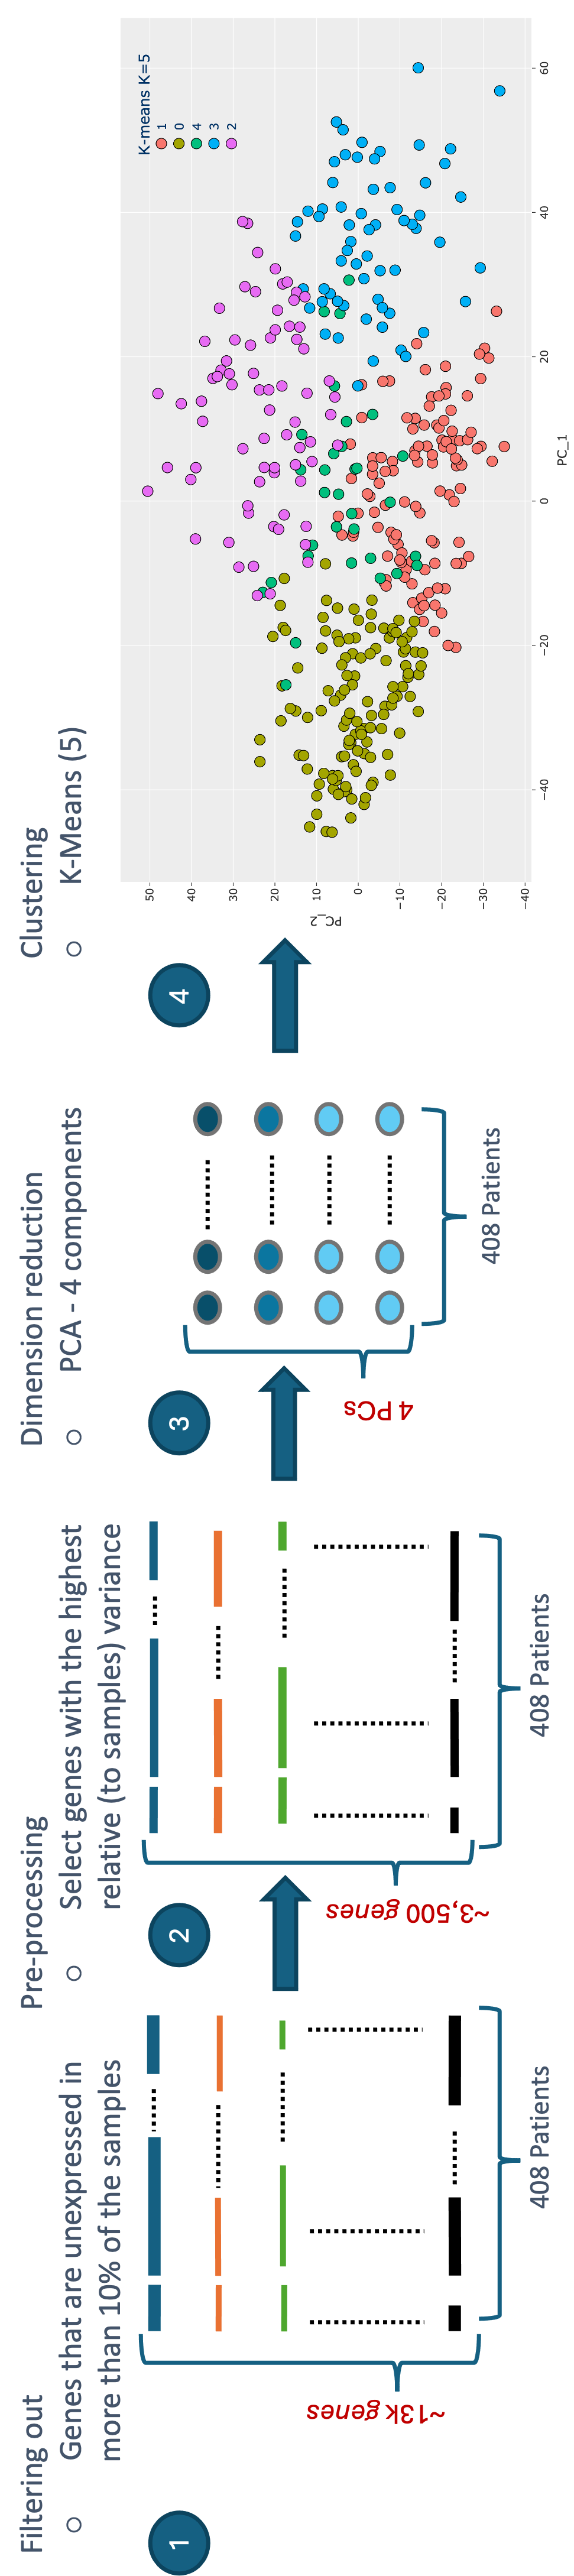
\includegraphics[width=1\textwidth,keepaspectratio]{Sections/ClusteringAnalysis/Resources/clustering_pipeline.png}
    \caption{Summary of the clustering analysis developed in this section}
    \label{fig:cs:clustering_pipeline}
\end{figure}

The clustering analysis established in this part of the thesis is simple using basic clustering and dimension reduction techniques. So far the approach taken was unbiased and the configurations were decided based on established clustering metrics. There was no domain knowledge used, apart from the guiding parameters for the numbers of genes to be kept from the TCGA's MIBC paper from \citet{Robertson2017-mg}. It can be noted that the number of clusters arrived is the same as in the above-mentioned work and that the consensus \citet{Kamoun2020-tj} found 6 subtypes. 

In the following section, the 5 clusters are explored in more depth and put in the context of the other work performed in the Jack Birch Unit \citet{Baker2022-bj}, TCGA \citet{Robertson2017-mg}, Lund classifier \citet{Marzouka2018-ge} and the consensus \citet{Kamoun2020-tj}. It will also cover their clinical implication by performing Kaplan-Meier survival analysis and Defferentialy Expressed Analysis (DEA).



